\pdfminorversion=4
\documentclass[aspectratio=169]{beamer}

\mode<presentation>
{
  \usetheme{default}
  \usecolortheme{default}
  \usefonttheme{default}
  \setbeamertemplate{navigation symbols}{}
  \setbeamertemplate{caption}[numbered]
  \setbeamertemplate{footline}[frame number]  % or "page number"
  \setbeamercolor{frametitle}{fg=white}
  \setbeamercolor{footline}{fg=black}
} 

\usepackage[english]{babel}
\usepackage[utf8x]{inputenc}
\usepackage{tikz}
\usepackage{courier}
\usepackage{array}
\usepackage{bold-extra}
\usepackage{minted}
\usepackage[thicklines]{cancel}
\usepackage{fancyvrb}

\xdefinecolor{dianablue}{rgb}{0.18,0.24,0.31}
\xdefinecolor{darkblue}{rgb}{0.1,0.1,0.7}
\xdefinecolor{darkgreen}{rgb}{0,0.5,0}
\xdefinecolor{darkgrey}{rgb}{0.35,0.35,0.35}
\xdefinecolor{darkorange}{rgb}{0.8,0.5,0}
\xdefinecolor{darkred}{rgb}{0.7,0,0}
\definecolor{darkgreen}{rgb}{0,0.6,0}
\definecolor{mauve}{rgb}{0.58,0,0.82}

\title[2018-09-18-jlab-reprise]{Data analysis tools from within HEP and from industry}
\author{Jim Pivarski}
\institute{Princeton University -- DIANA-HEP}
\date{September 18, 2018}

\usetikzlibrary{shapes.callouts}

\begin{document}

\logo{\pgfputat{\pgfxy(0.11, 7.4)}{\pgfbox[right,base]{\tikz{\filldraw[fill=dianablue, draw=none] (0 cm, 0 cm) rectangle (50 cm, 1 cm);}\mbox{\hspace{-8 cm}
\includegraphics[height=1 cm]{princeton-logo-long.png}
\includegraphics[height=1 cm]{diana-hep-logo-long.png}}}}}

\begin{frame}
  \titlepage
\end{frame}

\logo{\pgfputat{\pgfxy(0.11, 7.4)}{\pgfbox[right,base]{\tikz{\filldraw[fill=dianablue, draw=none] (0 cm, 0 cm) rectangle (50 cm, 1 cm);}\mbox{\hspace{-8 cm}
\includegraphics[height=1 cm]{princeton-logo.png}
\includegraphics[height=1 cm]{diana-hep-logo.png}}}}}

% Uncomment these lines for an automatically generated outline.
%\begin{frame}{Outline}
%  \tableofcontents
%\end{frame}

% START START START START START START START START START START START START START

\begin{frame}{The point I want to make}
\large
\vspace{0.5 cm}
\begin{itemize}\setlength{\itemsep}{0.25 cm}
\item Although nuclear and high energy physics once dealt with the world's largest datasets, this is no longer true. ``Big Data'' or (better) ``Web Scale'' analysis regularly deals with petabytes and exabytes, and they've developed software tools for it.

\item<2-> We can reduce maintenance costs and improve students' career options by mixing industry standard tools with our in-house tools, particularly for cases in which the purpose of the tool is the same.

\item<3-> This is in line with ROOT's new Python and TMVA interfaces, but broader: data should flow freely to the best tool for the job and back again, leaving the choice in the physicist's hands.
\end{itemize}

\uncover<4->{\textcolor{darkblue}{In short, we should become like other sciences, like astronomy or biology: common libraries for common stuff and our own libraries for domain-specific stuff.}}
\end{frame}

\begin{frame}{\only<1>{We measure globally distributed data in hundreds of PB}\only<2>{But for ``web scale'' companies, 100 PB = 1 truck}}
\vspace{0.35 cm}
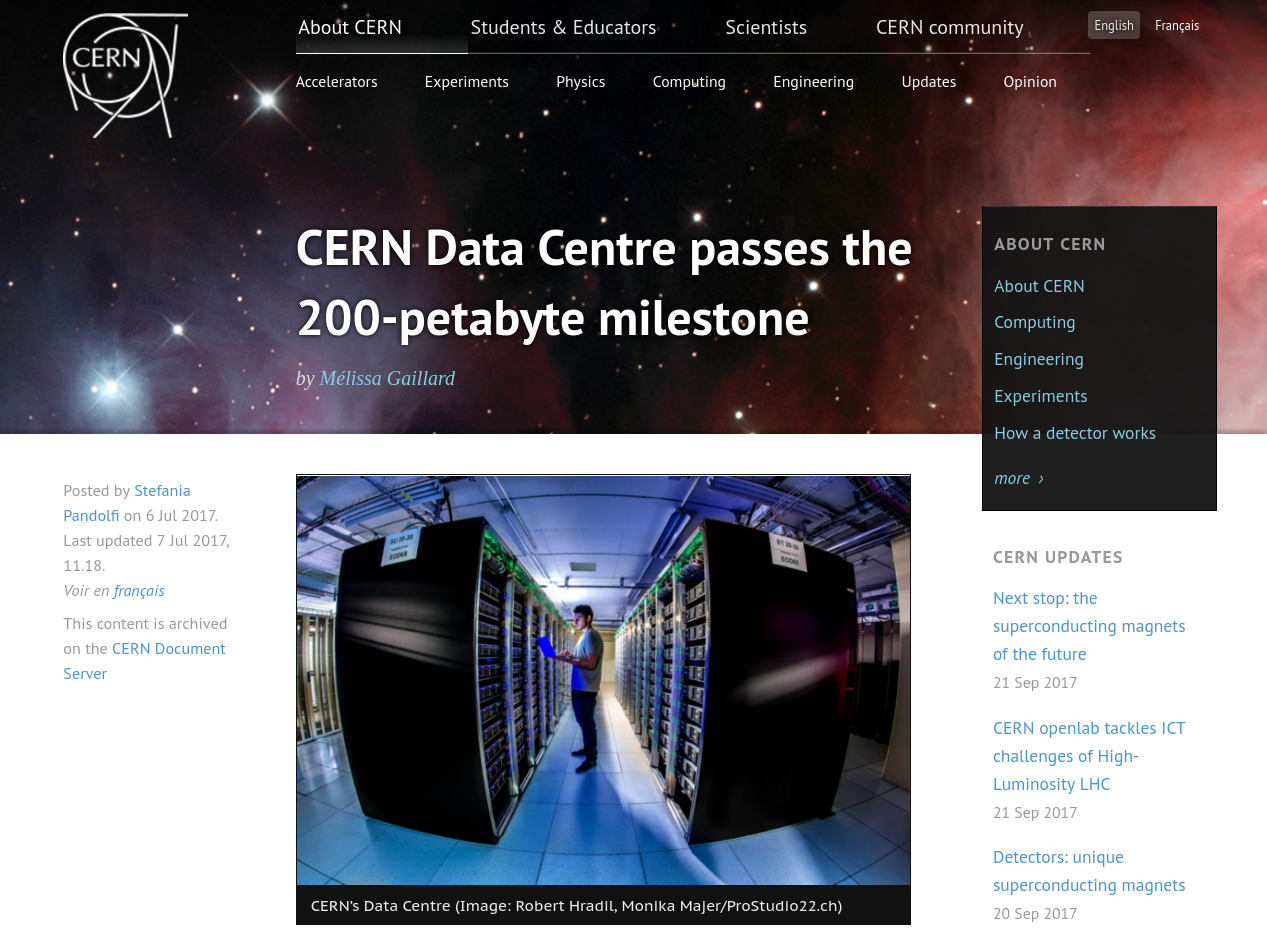
\includegraphics[width=0.73\linewidth]{cern-200pb.png}

\vspace{-4.8 cm}
\uncover<2->{\mbox{ } \hfill 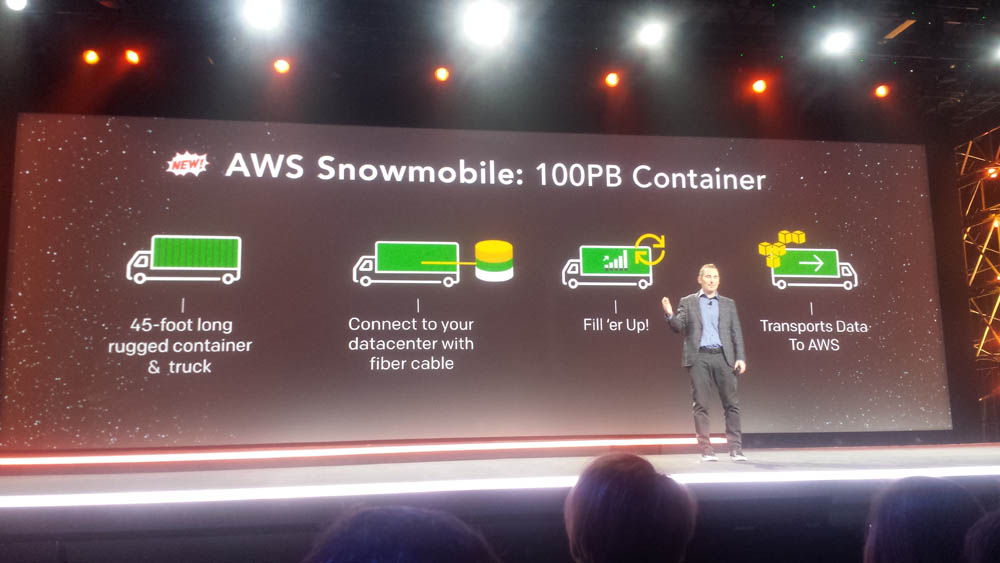
\includegraphics[width=0.7\linewidth]{aws-snowmobile.jpg}\hspace{-1 cm}}
\end{frame}

\begin{frame}{Number of people (users and developers) also dwarf our field}
\vspace{0.25 cm}
\mbox{ } \hfill 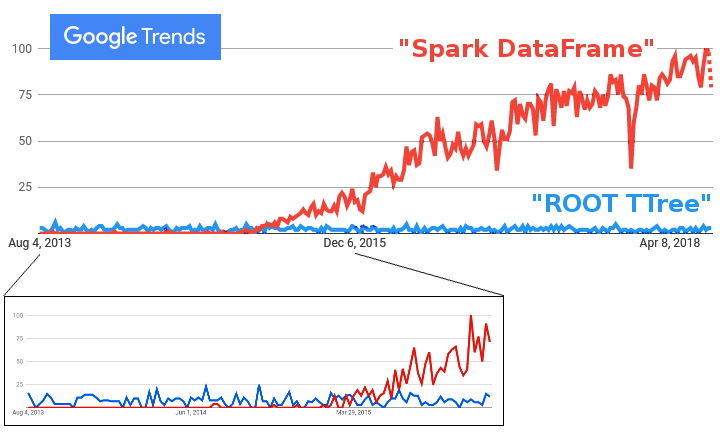
\includegraphics[width=0.9\linewidth]{root-spark-google-trends.png} \hfill \mbox{ }
\end{frame}

\begin{frame}{Number of people (users and developers) also dwarf our field}
\large
\vspace{0.5 cm}
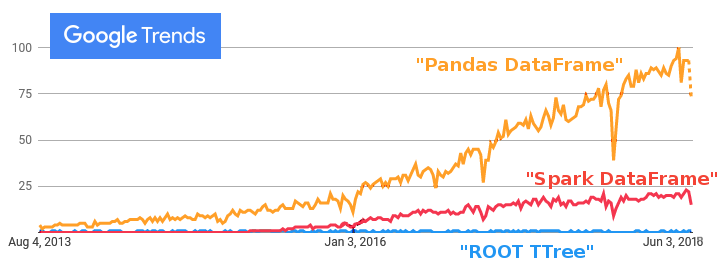
\includegraphics[width=\linewidth]{root-spark-pandas-google-trends.png}

\vspace{0.5 cm}
\uncover<2->{More users means more bug reports, more online help, more how-to blogs\ldots}

\vspace{0.2 cm}
\uncover<2->{More developers means more bug-fixes, more features, more connectors\ldots}
\end{frame}

\begin{frame}{Another important metric: experience!}
\Large
\vspace{0.25 cm}
\begin{itemize}\setlength{\itemsep}{0.25 cm}
\item Physicists have been performing big data analytics (reducing large datasets to statistical inferences) for about \textcolor{darkblue}{\underline{50 years}}.

\item Web scale companies have been doing it for about \textcolor{darkblue}{\underline{10 years}}.
\end{itemize}

\vspace{0.5 cm}
\uncover<2->{Nuclear and high-energy physics analysis is specialized and sophisticated--- many tools we'd call ``basic'' are not implemented in industry-grade software.}

\vspace{0.5 cm}
\uncover<3->{The simple prescription of ``just use Spark'' would leave analyzers without some necessary tools.}
\end{frame}

\begin{frame}{What should we do?}
\large
\vspace{0.5 cm}
\begin{columns}[t]
\column{0.25\linewidth}
\textcolor{darkblue}{\underline{Option \#1}}

\vspace{0.25 cm}
All of our needs are specialized.

\vspace{0.25 cm}
Continue developing our own everything.

\vspace{2.5 cm}

\column{0.25\linewidth}
\begin{uncoverenv}<2->
\textcolor{darkblue}{\hspace{-0.18 cm}\underline{Option \#2}}

\vspace{0.25 cm}
Modern big data software has some good ideas; integrate those \underline{\it ideas} into our stack.
\end{uncoverenv}

\column{0.25\linewidth}
\begin{uncoverenv}<3->
\only<3-4>{\textcolor{darkblue}{\hspace{-0.18 cm}\underline{Option \#3}}}\only<5->{\textcolor{darkorange}{\hspace{-0.18 cm}\underline{Option \#3}}}

\vspace{0.25 cm}
\only<3-4>{Narrow our scope to domain-specific tools, what no one else is developing, and make them interoperate with non-physics tools for the common parts.}\only<5->{\textcolor{darkorange}{Narrow our scope to domain-specific tools, what no one else is developing, and make them interoperate with non-physics tools for the common parts.}}
\end{uncoverenv}

\column{0.25\linewidth}
\begin{uncoverenv}<4->
\textcolor{darkblue}{\hspace{-0.18 cm}\underline{Option \#4}}

\vspace{0.25 cm}
Convince the world to start using physics analysis techniques so that they will develop solutions for these, too.
\end{uncoverenv}
\end{columns}

\vspace{0.5 cm}
\uncover<5->{\textcolor{darkorange}{\bf \#3 is my opinion, but what's domain-specific and what's not?}}
\end{frame}

\begin{frame}{Three examples each:}
\Large
\vspace{-0.5 cm}
\begin{columns}[t]
\column{0.5\linewidth}
\mbox{\hspace{0.25 cm}\textcolor{darkblue}{\underline{What web scale software's got}}}

\vspace{0.25 cm}
\begin{enumerate}
\item Distributed DAG processing
\item Indexed analysis
\item Machine learning
\end{enumerate}

\column{0.5\linewidth}
\mbox{\hspace{0.45 cm}\textcolor{darkblue}{\underline{What we need that it hasn't got}}}

\vspace{0.25 cm}
\begin{enumerate}
\item Nested data structures
\item Advanced histogramming
\item Ansatz fitting
\end{enumerate}

\end{columns}
\end{frame}

\begin{frame}{}
\huge
\vspace{0.5 cm}
\begin{center}
\textcolor{darkblue}{Distributed DAG processing}

\large
\vspace{0.5 cm}
not HEP-specific
\end{center}
\end{frame}

\begin{frame}{Distributed DAG processing}
\large
\vspace{0.5 cm}
\begin{columns}
\column{0.21\linewidth}
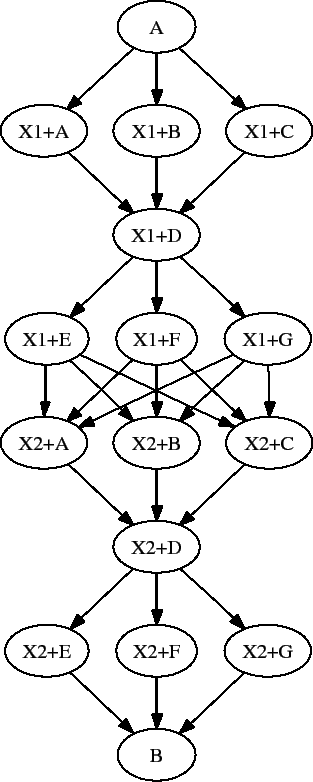
\includegraphics[width=\linewidth]{dag-htcondor.png}

\column{0.83\linewidth}
DAG: Directed Acyclic Graph of dependencies between subtasks.

Some would say this is what big data processing \underline{\it is}.

\vspace{1 cm}
Many frameworks distribute work this way:

\vspace{0.2 cm}
\hfill \begin{minipage}{0.95\linewidth}
\textcolor{darkblue}{Spark} (JVM), \textcolor{darkblue}{Dask}, \textcolor{darkblue}{Joblib}, \textcolor{darkblue}{Parsl} (Python), \textcolor{darkblue}{Storm} (continuous), \textcolor{darkblue}{Thrill} (C++), \textcolor{darkblue}{DAGMan} (HTCondor), \textcolor{darkblue}{TensorFlow} (fitting)\ldots
\end{minipage}

\vspace{1 cm}
Physics software is embracing this approach:

\begin{itemize}
\item RDataFrame in ROOT
\item Dozens of examples at CHEP
\end{itemize}
\end{columns}
\end{frame}

\begin{frame}{RDataFrame from the ROOT Workshop (last week)}
\vspace{0.25 cm}
\only<1>{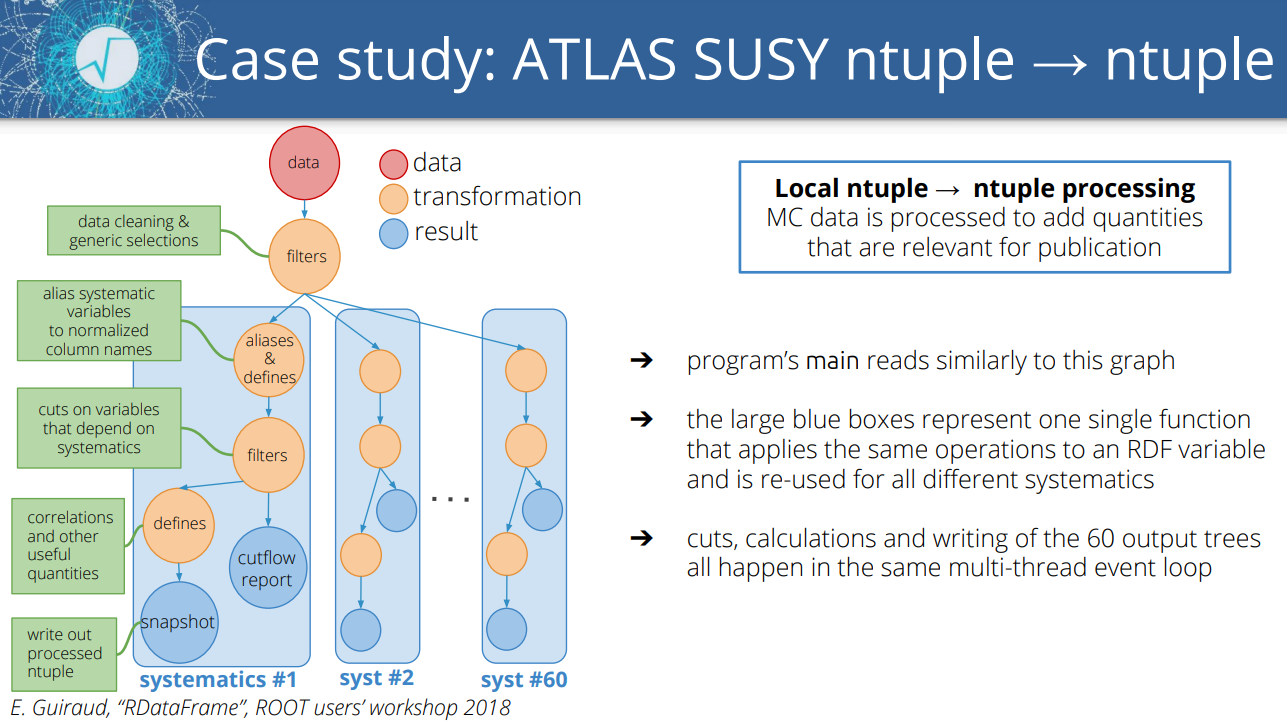
\includegraphics[width=\linewidth]{rdataframe-use-case-1.png}}
\only<2>{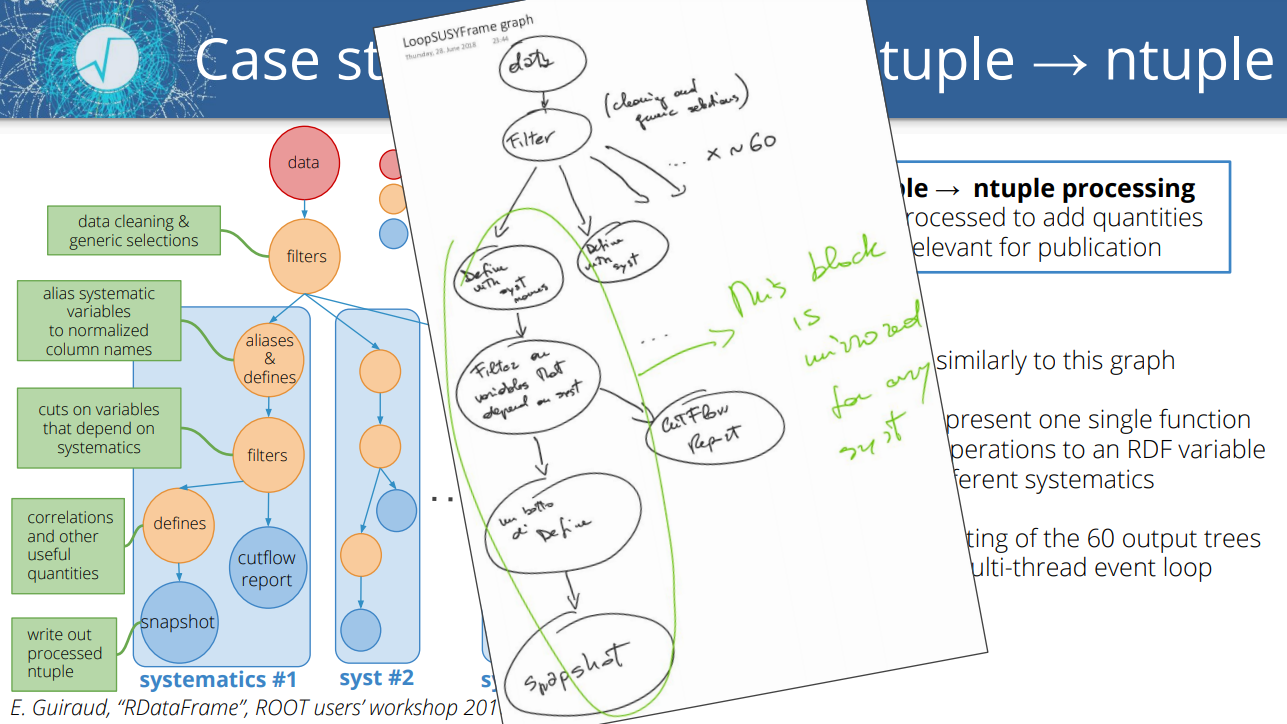
\includegraphics[width=\linewidth]{rdataframe-use-case-2.png}}
\end{frame}

\begin{frame}{But how will it develop?}
\Large
\vspace{0.5 cm}
\begin{columns}
\column{0.9\linewidth}
Will RDataFrame be a {\it programming model} that {\it interfaces} with distributed processing systems such as Spark?

\vspace{0.5 cm}
Or will it be {\it part} of a ROOT {\it implementation} of distributed DAG processing? A new PROOF, for instance?
\end{columns}

\vspace{1 cm}
\uncover<2->{\textcolor{darkblue}{Distributing computational tasks with dependencies is a good example of a non-domain-specific problem.}}
\end{frame}



\end{document}
